\chapter{Introduction}
%
\label{chap:intro}
%
\section{Background}
In modern days, the high patient influx and the proliferation of medical image acquisition have exponentially increased the workload for medical professionals examining diagnostic images. Furthermore, the precision demanded in these analyses necessitates extensive training and expertise spanning over several years. In this context, artificial intelligence (AI) and machine learning (ML), specifically deep neural networks (DNNs), emerge as promising solutions to alleviate this burden on medical practitioners. In the realm of modern DNNs, significant strides have been made to attain expert human performance across various medical imaging challenges, such as medical image reconstruction, noise reduction, quality assurance, triage, segmentation, computer-aided detection, and classification \cite{fan2020pranet, huber2022dedicated, kretz2020mammography, shen2019deep, wang2020deep, wang2018interactive, wu2021drone, yala2019deep}. Recently DNNs have shown exceptional capabilities in various cancer detection tasks, such as effectively identifying breast cancer, lung cancer, pancreatic cancer, and melanoma \cite{ardila2019end, bejnordi2017diagnostic, chu2019application, codella2017deep, coudray2018classification, han2017breast, li2018skin, roth2015deep, wang2016deep}. Leveraging DNNs holds the potential to significantly enhance the accuracy of assessments by radiologists \cite{choy2018current}. The growing consensus is that AI algorithms are poised to revolutionize clinical imaging practices in the coming decade.

%% Add details on imaging modalities -- and some background on MIC tasks.

\begin{figure}[!t]
\centering
	\begin{subfigure}[b]{0.5\linewidth}
	\centering
	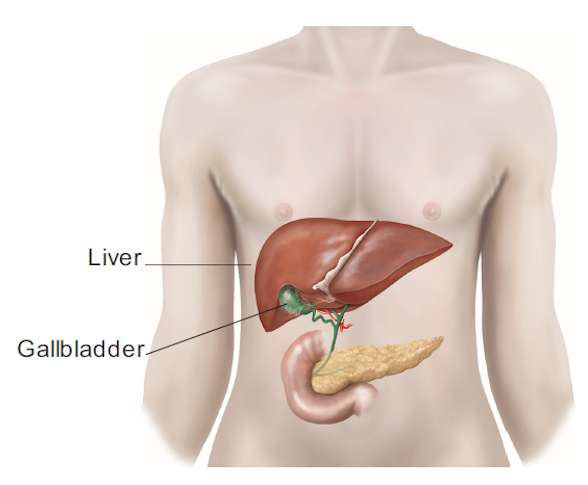
\includegraphics[width=\linewidth]{figs/gallbladder.png}
		\caption{}
		\label{fig:gb_whole}
	\end{subfigure}
	%
	\begin{subfigure}[b]{0.32\linewidth}
	\centering
	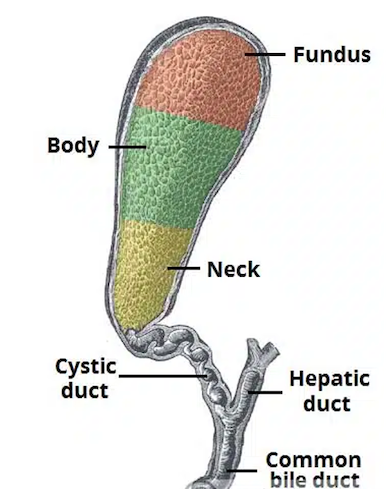
\includegraphics[width=\linewidth]{figs/gb_anatomy.png}
		\caption{}
		\label{fig:gb_anatomy}
	\end{subfigure}
	%
	\caption[Anatomy of Gallbladder in the human body]{(a) Anatomical positions of gallbladder and Liver in the human body. Image courtesy: Department of Health, Western Australia \cite{gb_image}. (b) The anatomical structure of the gallbladder including the three parts -- fundus, body, and neck.}
    \label{fig:gb}
\end{figure}

\par Inspired by the recent success of DNNs in medical imaging tasks, we systematically delve into the challenges involved in detecting Gallbladder Cancer (GBC) from diagnostic Ultrasound (USG). The Gallbladder (GB) is a hollow, pear-shaped and balloon-like gastrointestinal organ filled with bile juices and resides just under the liver. GB is found in the upper-right part of the abdomen. The anatomical structure of a GB consists of three parts -- (1) \emph{fundus}, the large rounded base that stores the bile, (2) \emph{body}, the tapered portion after fundus, and (3) \emph{neck}, the narrow and tapered area which joins with cystic duct. \cref{fig:gb} shows a pictorial overview of the anatomical position of the GB in the human body. Due to the contiguous tissues of GB with the liver, the malignancy in GB can quickly spread to the liver, adjacent organs, and lead to distant metastases (cancer spreading to distant organs). %The metastasis of gallbladder cancer can extend to neighboring tissues, organs, the entire abdominal cavity, or distant regions within the body. 
Despite previous efforts in the segmentation and detection of Gallbladder (GB) afflictions, such as detecting stones and polyps \cite{gbPolyp, gbPolyp2, gbAutomatic}, there is a noticeable gap in research concerning the application of DNNs for the detection of GBC. A search on Google Scholar with the keywords ``artificial intelligence'' and ``gallbladder cancer'' returned 204 articles between January 2015 and November 2021. In these, we did not find any published article on deep learning-based \gbc detection from \usg images. This gap emphasizes the need for further exploration into the utility of advanced neural network models in GBC detection, promising advancements in early diagnosis and improved patient outcomes. In the following sections, we discuss the implications and the motivation behind the study. 


\begin{figure}[t]
    \centering
    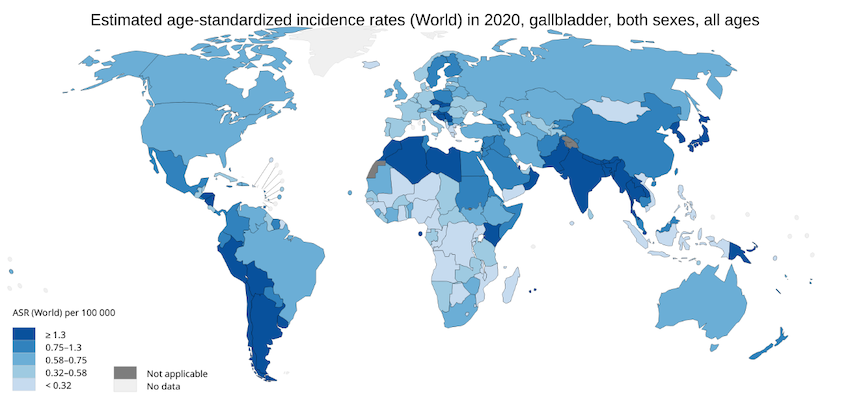
\includegraphics[width=0.8\linewidth]{figs/asr-map.png}
    \caption[The worldwide Age Standardized Incidence Rates (ASR) of GBC]{The worldwide Age Standardized Incidence Rates (ASR) of GBC. India sees a very high ASR, and is facing a significant risk of GBC. Image courtesy: GLOBOCAN \cite{bray2018global}.}
    \label{fig:asr_worldmap}
\end{figure}

\section{Gallbladder Cancer and its Risks}
%
\subsection{Gallbladder Cancer} 
% %
Gallbladder Cancer is an abnormal growth of cells that begins in the gallbladder. GBC is the most common biliary tract cancer and the fifth most common malignancy of the gastrointestinal tract \cite{HBSN4726}. According to GLOBOCAN 2020 data, GBC causes 84,695 deaths and 1,15,949 incidences every year worldwide \cite{armitage2014abeloff, bray2018global}. The disease is among the very few types of cancers which manifest a higher proportion of mortality than incidence \cite{bray2018global}. GBC has a very high mortality rate with 5-year survival rate of less than 5\% in patients with advanced disease.
The treatment involves surgically removing the GB and parts of surrounding regions from the hepatobiliary system when the malignancy is localized to GB and its wall. The surgical resection can also be followed with radiation or chemotherapy. For metastasized GBC, curative resection is infeasible, as the cancer has already spread to distant organs. GBC is overly deadly because it is rarely detected before an advanced and metastasized stage in most patients \cite{batra2005gallbladder, randi2006gallbladder}. 

%% Expand slightly

\subsection{Risks of GBC} 
% %
GBC is prevalent in China, India, and Latin America according to GLOBOCAN data \cite{bray2018global}. India, specifically, experiences a significant rise in Gallbladder Cancer (GBC). The incidence rate of GBC in India matches the globally highest rates. \cref{fig:asr_worldmap} shows the age-standardized incidence rates of GBC in different countries across the globe.
Furthermore, Indian patients contribute to more than 20\% of the annual mortality associated with Gallbladder Cancer (GBC). GBC also stands out as a leading cause of cancer-related deaths among Indian women \cite{randi2006gallbladder}. GBC is often detected at an advanced and metastasized stage for most patients, impeding curative resection and resulting in a dismal prognosis \cite{gupta2021locally, randi2006gallbladder}. 
%In fact, medical practitioners discover GBC by chance after a GB surgery in most cases. 
In the USA, only about 1 in every 5 cases of GBC are identified in an early stage \cite{howlader2017seer}. Although, early diagnosis provides an excellent chance to combat the disease by surgical removal, such timely diagnosis, unfortunately, is rare. The overall mean survival rate for patients with advanced GBC is six months, with a 5-year survival rate of 5\% \cite{levy2001gallbladder}. The median survival of patients with suspected GBC is 9.2 months, and 26.5 months for patients with incidental diagnosis \cite{wullstein2002complications}. Although GBC is relatively rare, its high mortality rate signifies the criticality of early diagnosis to improve the survival statistics of the deadly disease.  

\section{Motivation of the Study}
%
Early diagnosis and timely resection play a critical role in improving the survival rate of GBC. Studies indicate that the 5-year survival rate could be enhanced to 44\% with prompt medical interventions \cite{chen2016long}. USG is the most commonly used non-invasive diagnostic imaging method due to its non-ionizing radiation, portability, low cost, and widespread availability \cite{klibanov2015ultrasound}. Especially in India, Computed Tomography (CT) and Magnetic Resonance Imaging (MRI) are primarily accessible in tertiary care hospitals in big cities, and cost about ten times more than USG. Further, CT uses multiple X-ray images obtained from various angles to generate detailed cross-sectional images of the internal structures within the body, and thus expose the patients to X-ray radiation. USG is usually the de facto choice of diagnostic modality in low-resource settings, and serves as the primary imaging test for assessing GB diseases and is often the sole diagnostic tool for patients with suspected GB ailments. If no malignancy is suspected during the initial screening, further testing is usually not conducted, allowing GBC to progress silently. Surgical removal of GBC becomes infeasible at advanced stages.

\par Timely detection of GBC is crucial for enabling patients to undergo surgical and therapeutic interventions, ultimately improving the prognosis of the disease. Given that USG is the predominant diagnostic imaging modality for abdominal ailments, enhancing its ability to detect GBC would facilitate early diagnosis and contribute to improving survival statistics. Detecting signs of GBC through USG would provide healthcare professionals with a valuable tool for prompt intervention and treatment planning. The motivation of this work is leveraging the accessibility and widespread use of USG to enhance its effectiveness in identifying GBC (including accidental detections), thus positively impacting patient outcomes and survival rates.  

\section{Challenges of using Ultrasound}
%
Ultrasound (USG) operates by emitting high-frequency sound waves, typically in the range of 2--20 megahertz (MHz), from a transducer probe into the body. These sound waves travel through the body and bounce back (echo) when they encounter tissue boundaries or organs with different densities. The returning echoes are then detected by the transducer and converted into electrical signals, which are processed by a computer to generate real-time images of the internal structures. By analyzing the strength and timing of these echoes, ultrasound technology can create detailed images of organs, tissues, and blood flow without using ionizing radiation, making it a safe and non-invasive imaging modality. \cref{fig:usg_sample} shows USG images of the gallbladder. 
In \Cref{chap:usg} we provide more details on ultrasound imaging, the noise and artifacts inherent to ultrasound, and the relevant terminologies.


\begin{figure}[t]
    \centering
    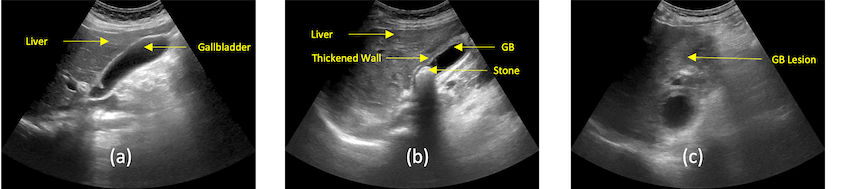
\includegraphics[width=0.95\linewidth]{figs/usg_sample.png}
    \caption[Ultrasound image samples]{USG image samples of the gallbladder (GB). (a) A normal GB along with the adjacent liver. (b) A GB with benign wall thickening and stone. (c) Malignant lesion at the GB.}
    \label{fig:usg_sample}
\end{figure}


Although USG is the primary diagnostic tool for assessing GB diseases, identifying the malignancy in routine USG remains a formidable challenge due to factors such as similar visual appearance with benign diseases, or confounding medical conditions (refer to \cref{sec:clinical}). Expert radiologists, even with years of experience, struggle to achieve more than 70\% sensitivity in GBC detection, indicating the need for more robust diagnostic methodologies.  Furthermore, the application of DNNs to analyze USG images faces significant hurdles, primarily stemming from the unique characteristics of USG imaging. USG images suffer from low quality due to noise, artifacts like shadows, and spurious textures, which can bias DNN classifiers and compromise detection accuracy. The handheld nature of ultrasound sensors introduces operator-specific visual variations across radiologists and medical centers, further complicating GBC detection. Further, malignant GB often presents irregular anatomy and low inter-class variability, making it challenging to distinguish from benign conditions. Moreover, the absence of well-annotated datasets poses a significant challenge for developing and training accurate DNN models for GBC detection, hindering progress in the field. We provide a detailed discussion about  challenges of using USG for GBC detection along with visual examples in \Cref{sec:challenges}. 


\section{Key Research Objectives}
%
The key research objectives of this thesis are as following:
\begin{itemize}
    \item Address the challenges posed by Ultrasound images, including noise, shadow, and spurious textures in detecting GBC and enhance the accuracy of GBC predictions by DNN models. 
    %
    \item Investigate techniques for learning from limited supervised data, particularly considering the scarcity of specialized annotations for medical data. Explore methods to leverage unlabelled or weakly labelled data for superior performance in GBC detection.
    %
    \item Explore methods to incorporate interpretability into model decision-making processes. Aim for models that provide insights into how predictions are reached, fostering better compatibility for clinical usage.
    %
    \item Assess the effectiveness of using Ultrasound video data directly for identifying GBC. Video-based detectors also eliminate the necessity for radiologists to select frames for GBC detection manually, reducing the effect of operator variability. 
    %
    \item Collect and curate annotated dataset in the form of both ultrasound images and videos to benefit the community. 
\end{itemize}



\section{Organization of Subsequent Chapters}
%
The thesis is organized into the following subsequent chapters:
    %\item \underline{Chapter I}: Introduction, providing a comprehensive overview of the research endeavor. The chapter outlines the problem statement, the motivation behind the study, the challenges, and the key research objectives that set the stage for subsequent chapters. 

\mypara{\Cref{chap:usg}} We briefly discuss the fundamentals of the Ultrasound imaging modality, and the issues and challenges associated with developing computer assisted methods for diagnosis of GBC from USG.  

\mypara{\Cref{chap:data}} In this chapter, we focus on the data used in this study and discuss the acquisition, curation, annotation, and statistics related to the data. 

\mypara{\Cref{chap:gbcnet}} We address the challenges associated with Ultrasound imaging, such as noise and artifacts, and provide the details of developing an accurate Gallbladder Cancer (GBC) detection model. An innovative classification model and a novel smoothing-based curriculum were the key technical contributions towards this end.
    
%\mypara{\Cref{chap:limited}} This chapter is centered on the issue of learning from limited supervised data, and investigates two distinct strategies -- (1) leverage unlabelled video data for achieving superior performance in downstream GBC detection, and (2) use weak image-level labels instead of the dense bounding box labels to train a GBC detector.

\mypara{\Cref{chap:limited}} This chapter is centered on the issue of learning from limited supervised data, and discusses how to leverage unlabelled video data for achieving superior performance in downstream GBC detection.

\mypara{\Cref{chap:wsod}} In this chapter, we present another alternative approach to learning from limited supervised data. We use weak image-level labels instead of the dense bounding box labels to train a GBC detector.

\mypara{\Cref{chap:radformer}} We investigate the development of explainable solutions for GBC detection in this chapter. The chapter critically analyzes interpretability in the context of model outputs, contributing to the broader understanding of decision-making processes.

\mypara{\Cref{chap:focusmae}} This chapter introduces and elucidates comprehensive video-based detection techniques. It explores the advantages and challenges of transitioning from images to video-based detection methods.

\mypara{\Cref{chap:conclusion}} The chapter serves as a conclusion, notes the limitations, and assesses the current and future scope of the work. We identify the potential avenues for further exploration and development and provide a roadmap for future advancements.
